\documentclass[11pt,a4paper]{article}
\usepackage[show]{ed}
\usepackage{tikz}
\usepackage{float}
\usepackage{hyperref}
\usepackage[style=alphabetic, backend=bibtex]{biblatex}
\usepackage{graphicx}

\title{Building MathHub using React\\ \vspace{2 mm} Bachelor Thesis}
\author{Johannes-Sebastian See\\Supervisor: Michael Kohlhase\\Co-supervisor: Tom Wiesing\\Friedrich-Alexander University, Erlangen Nürnberg, Germany}

\date{\today}
\addbibresource{local.bib}

\providecommand\myxscale{.95}
\providecommand\myyscale{1}

\begin{document}

\begin{titlepage}
\maketitle
\begin{abstract}
Abstract will be added at the end
\end{abstract}

\end{titlepage}

\tableofcontents
\section{Introduction}
\subsection{Math Information Systems}
\ednote{why are those special and different}
\ednote{System to impart mathematical knowledge to people}
\subsection{MathHub}
\subsection{Previous Implementation}
Up until April 2018 the MathHub frontend was realized with Drupal.
Drupal is an open source content-management framework used by millions of different websites.
User interactions were handled by JavaScript modules in the JOBAD framework \cite{comp}.
	
But in April 2018 a critical security flaw in the versions 6 to 8 went public.
The problem was that Drupal in these versions accepts request parameters without any validation.
This means it processes any input from anybody \cite{zdnet}.
To exploit this weakness an attacker doesn't even need to log in or have any other privileges on a vulnerable website \cite{register}.
With this flaw it is possible to inject malicious code and compromise a website in multiple ways.
This can be used to access, change and delete private data and create backdoors to make future attacks possible.
The Drupal community called this weakness "Drupalgeddon2" while its official name was "CVE-2018-7600".
Some code that was injected installed the program XMRig Monero miner, which is a cryptocurrency mining program, as well as deleting other mining programs on the compromised system \cite{hacker}.
The National Institute of Standards (NIST) and Technology gave Drupal a "Highly Critical" Rating because of this vulnerability \cite{nist}.
 After this flaw was discovered a patch was published and a warning to update every website that used a vulnerable version was given.
	
Since there have been multiple flaws in Drupal before that compromised MathHub, the decision to stop using it and rebuild MathHub from the ground up to not be affected by future attacks, was made. \ednote{This is too much detail. Shorten this}

\begin{itemize}
\item give a preview
\item we need MathHub
\item use a Frontend
\item list sections
\end{itemize}
\section{State of the art}
\subsection{Math Information Systems}
\begin{itemize}
\item Zentral Blatt Math
\item mlfdb
\item Wolfram alpha
\item isu-afp.org
\item mathoverflow: Q{\&}A site for mathematicians to discuss unsolved math problems
\item Wikidata: central storage for Wikimedia
\item Wikipedia: part of Wikimedia
\item what can they do? what is their goal? what can we do different/better?
\end{itemize}

\subsection{Building an interactive Frontend} \ednote{list some differences between the frameworks}
Before starting to build a completely new MathHub frontend a different web framework had to be chosen.

\textbf{Polymer} \cite{polymer} is an open source JavaScript library developed and maintained by Google.
It provides a set of features that make creating custom elements, that work like standard web components, easy.
It is used for several Google services for example Youtube, Google Earth, Google Play Music etc. as well as Netflix, Electronic Arts and many other companies. \ednote{native support in Chrome}

Another open source web framework from Google is \textbf{Angular}. \cite{angular}
This TypeScript library has framework architectures that simplifies the development of new web applications.
It also has Angular Material.
A collection of UI components that work in browsers, on mobile and desktop.

After using Angular on several Google projects, Evan You decided to create his own JavaScript framework called \textbf{Vue.js} \cite{vuewiki}
Depending on the project it can be scaled between a framework and a library.
Vue.js separates its view layer library from its support libraries for complex applications, to create an easy approach to the framework. \cite{vuegit}

In the end the decision was made to use \textbf{React} developed by Facebook. \ednote{why?}
Further details about React and how it is used can be found in section \ref{preliminaries}. \ednote{short indtroduction before ref}


\section{Preliminaries} \label{preliminaries}
\subsection{The core concept of React} 
React is an open source JavaScript library owned and maintained by Facebook.	It was created to build interactive user interfaces (UI).
For example it is used for Facebook and Instagram.
What makes React unique is its use of a virtual Document Object Model (DOM). \ednote{Reference model view controller}
The concept of the virtual DOM is that when updating a website not everything is rendered again.
React computes the differences between the last and the next page and only changes the necessary parts.
On top of that it has conditional rendering which means that an item will only be rendered if it is shown.
The advantage of virtual and conditional rendering is that this makes updating a website fast, but it comes with high RAM costs.
The actual interface is made up of many different elements and components.
Since a website that uses React can have many different features it is helpful to build new components.
\cite{reactjs}
React does not have a styling system so it integrates \ednote{React does not intigrate this} Semantic UI to provide a consistent theme for the frontend.
\ednote{react does not force any styling system. We just use semantic-ui-react bindings}

\subsection{Building new components in React}
React already has a large library \ednote{external} with a lot of different components \ednote{clarify that components are node blocks of the virtual dom}, but it is often necessary to make new ones that have the desired functionality.
In JavaScript new components can be implemented by creating either a function or a class.
Their input variables are called props and can only be read.
Components return React elements that are ready to be rendered. \ednote{In: props; state; out: children of the tree => real leves:DOM}
Naturally a component can grow big rather quickly.
Luckily it is possible to use components inside other components.
This comes with the advantage that they can be reused in many different locations.
The difference between creating a new component as a function and as a class is that a class can have a private internal state, which can be updated an any time. \ednote{not relevant}
Since props are read-only, updating the state can only affect lower components.
If it is necessary to also change something in a higher component it is possible to "lift up" the state.
This means adding the state that causes the change to the state of the component on a higher level and giving it back to the lower levels as a prop.
If the update should affect a component on the same level creating a new component with that state that consist of all the one that are affected will  make this possible.
\cite{reactjsGS}

\subsection{MMT and OMDoc}
The abbreviation MMT is short for either \underline{m}eta-\underline{m}eta-\underline{t}heory or \underline{m}eta-\underline{m}eta-\underline{t}ool.
Whereby meta-meta-theory represents the theoretical and meta-meta-tool the practical part of MMT.
It is a knowledge representation framework that uses formal \ednote{ + informal, language independent} languages to create a scalable module system for mathematical theories.
That means that in MMT the features of the syntax and the semantics of a language are defined as individual, reusable modules.
This way of building individual languages leads to a high degree of abstraction of advanced algorithms.

MMT integrates \ednote{it uses OMDoc representation} the OMDoc format, which is a XML format \ednote{general format for which we use XML} that describes a design for an uniform language for knowledge.

\begin{figure}[H]
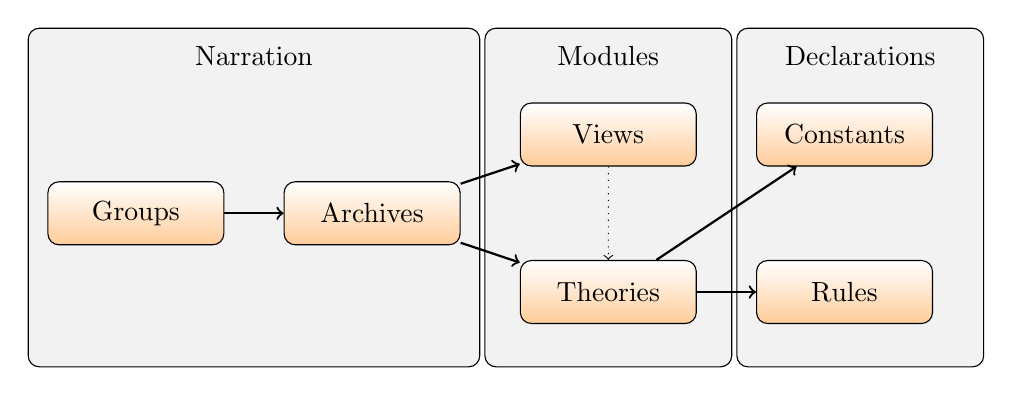
\begin{tikzpicture}[xscale=\myxscale, yscale=\myyscale]
  \tikzstyle{component} = [rectangle, draw, fill=orange!20, text width=2cm, text centered,
                                    rounded corners, minimum height=.8cm,shade, 
                                    top color=white, bottom color=orange!40]
  \tikzstyle{back} = [rectangle, draw, fill=gray!10, text width=2cm,
                                    rounded corners, minimum height=4.3cm]
\node[back, text width = 5.5cm,  label ={[shift={(0ex,-4ex)}]north:Narration}] (nar) {};
\node[back, right of =nar, xshift=3.5cm, text width = 2.9cm,  label ={[shift={(0ex,-4ex)}]north:Modules}] (mod) {};
\node[back, right of =mod, xshift=2.2cm, text width = 2.9cm,  label ={[shift={(0ex,-4ex)}]north:Declarations}] (dec) {};
\node[component, left of =nar, xshift=-0.5cm, yshift=-0.2cm] (groups) {Groups};
\node[component, right of =groups, xshift=2cm] (archives) {Archives};
\node[component, right of =archives, xshift=2cm, yshift=-1cm] (theo) {Theories};
\node[component, right of =archives, xshift=2cm, yshift=1cm] (views) {Views};
\node[component, right of=theo, xshift=2cm, yshift=2cm] (con) {Constants};
\node[component, right of=theo, xshift=2cm] (rul) {Rules};
\draw[->, thick] (groups) -- node[above]{} (archives);
\draw[->,thick] (archives) -- node[above]{} (theo);
\draw[->,thick] (archives) -- node[above]{} (views);
\draw[->,thick] (theo) -- node[above]{} (rul);
\draw[->,thick] (theo) -- node[above]{} (con);
\draw[->,dotted] (views) -- node[above]{} (theo);
\end{tikzpicture}
\caption{The MMT structure}
\end{figure}


To create a frontend that displays MMT it is important to understand its structure.
First up on the highest level are the individual groups.
Each group contains several archives.
An archive can be described as a software project that provides a work flow for a language in MMT. \ednote{group of document that typically are equivalent to a project}
Groups and archives are just used for navigation and narration purposes.
The modules that can be found in an archive, make up the actual content.
These are either a theory or a view that shows the relation between different theories.
A theory is defined by its rules and constants, the so called declarations. \ednote{can be seen in figure ...}
\cite{mmt}
 
\section{The Architecture of MathHub}

\subsection{MathHub.info Routes}
\begin{figure}[h]
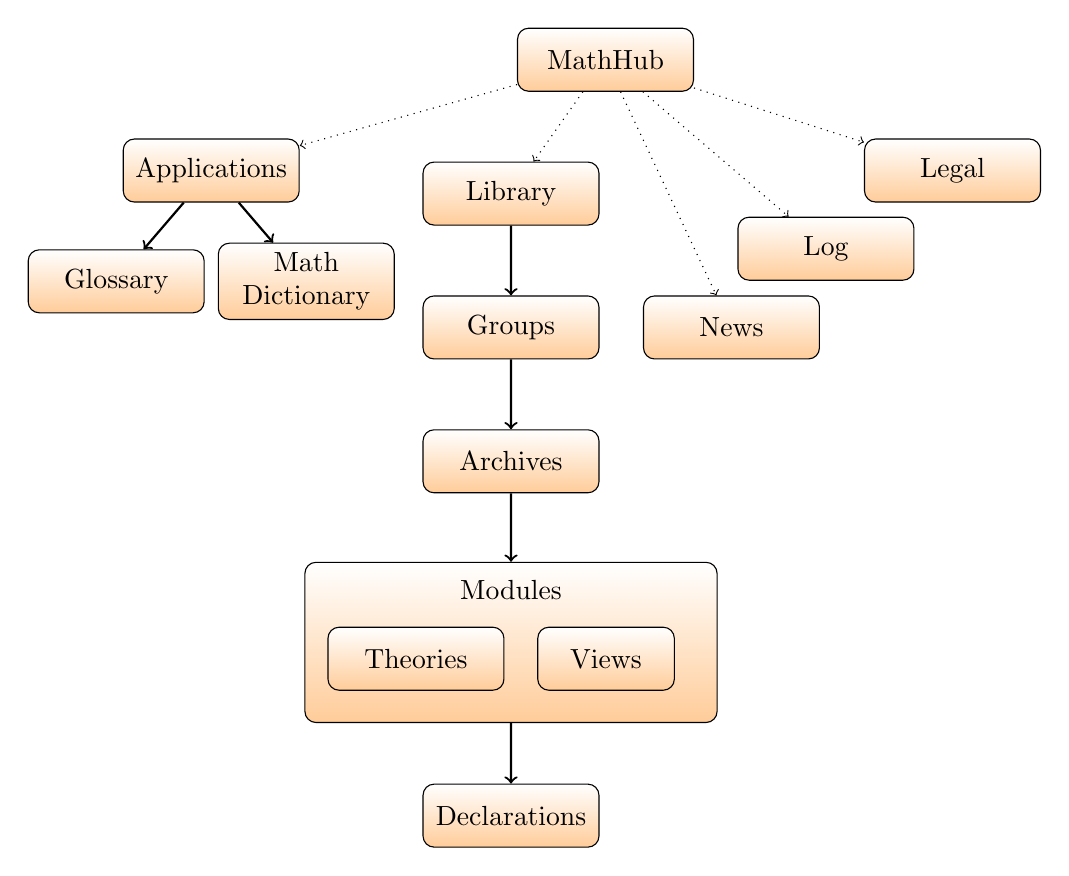
\begin{tikzpicture}[xscale=\myxscale, yscale=\myyscale]
  \tikzstyle{component} = [rectangle, draw, fill=orange!20, text width=2cm, text centered,
                                    rounded corners, minimum height=.8cm,shade, 
                                    top color=white, bottom color=orange!40]
                                   
\node[component] (MH) {MathHub};
\node[component, below of =MH, xshift=-1.2cm, yshift=-0.7cm] (lib) {Library};
\node[component, below of =lib, yshift=-0.7cm] (groups) {Groups};
\node[component, below of =groups, yshift=-0.7cm] (archives) {Archives};
\node[component, below of =archives, text width=5cm, text height=1.8cm, yshift=-1.3cm, label ={[shift={(0ex,-4ex)}]north:Modules}] (mod) {};
\node[component, below left of =mod, xshift=-0.5cm, yshift=0.5cm] (theo) {Theories};
\node[component, below right of =mod, text width=1.5cm, xshift=0.5cm, yshift=0.5cm] (views) {Views};
\node[component, below of=mod, yshift=-1.2cm] (decl) {Declarations};
\node[component, below left of =MH, xshift = -4.3cm, yshift=-0.7cm] (apps) {Applications};
\node[component, below left of =apps, xshift=-0.5cm, yshift=-0.7cm] (glos) {Glossary};
\node[component, below right of =apps, xshift=0.5cm, yshift=-0.7cm] (dict) {Math Dictionary};
\node[component, below of=MH, xshift=1.6cm, yshift=-2.4cm] (news) {News};
\node[component, below of=MH, xshift=2.8cm, yshift=-1.4cm] (log) {Log};
\node[component, below right of=MH, xshift=3.7cm, yshift=-0.7cm] (legal) {Legal};
\draw[->,dotted] (MH) -- node[above]{} (lib);
\draw[->,dotted] (MH) -- node[above]{} (apps);
\draw[->,dotted] (MH) -- node[above]{} (news);
\draw[->,dotted] (MH) -- node[above]{} (log);
\draw[->,dotted] (MH) -- node[above]{} (legal);
\draw[->,thick] (lib) -- node[above]{} (groups);
\draw[->, thick] (groups) -- node[above]{} (archives);
\draw[->,thick] (archives) -- node[above]{} (mod);
\draw [->,thick] (mod) -- node[above]{} (decl);
\draw[->,thick] (apps) -- node[above]{} (glos);
\draw[->,thick] (apps) -- node[above]{} (dict);
\end{tikzpicture}
\caption{MathHub components}
\end{figure}

To create a logical navigation system MathHub.info is divided into numerous pages, that can be accessed from the Home-page. \ednote{structured using routes}

\ednote{can be seen in figure ...} First of is the main content of MathHub, the MMT library.
It starts with the different groups.
The next page displays the archives that belong to a specific group.
Groups and archives exist only for narration and navigation purposes.
So they don't have any actual content only meta information like names and descriptions.
The actual content can be found in documents.
These document consist of several theories and views. \ednote{module + opaque}
So the archive-page has a list of all the documents in an archive.
On the document-page the modules are displayed with all their declarations.


With the huge mathematical library of theories there are a lot of technical terms.
The glossary is a collection of these expressions.
There wouldn't be much value in to just having a collection without any additional features.
So the glossary also provides a definition for each term.
Over the time many different authors have contributed to the theories, so it can happen that there are different terms that share a meaning.
These synonyms can also be found in the glossary.
Since many theories exist in multiple languages it makes sense to have a glossary available for every used language.
Currently the biggest collection of terms are in the English glossary, followed by German and French.
Smaller collections for Turkish and Romanian are also available as well as simplified and traditional Chinese. \ednote{cite smglom}

Most of the times a user does not want to browse through the gigantic glossary to just find a single term.
This is the reason why the Math Dictionary is a useful extension of the glossary.
The main purpose of the Math Dictionary is to translate a term into another language and look up a definition of a specific expression.


There is also a page with all the latest news regarding MathHub, as well as pages for licenses and the privacy policy. \ednote{couple of static pages}
At last there is a Log with the most recent messages from the backend.
\ednote{mention JSON (REST)}
\subsection{Layout}
Every page consists of three parts: A header, a footer and the actual content in between.

The header is a menu with the routes to Home, the news, the glossary and the Math Dictionary as well some external links.
Under the menu there are breadcrumbs for an easier navigation.
In the footer the logos of the institutions that are involved in MathHub can be found.
There also are the routes to the Log, the licenses, the imprint and the privacy policy.
The body itself depends on the page the user is currently on. \ednote{picture ref}
\begin{figure}[H]

\includegraphics[width=1\textwidth]{home.png}
\caption{The Homepage}
\end{figure}

\subsection{Realization}
\ednote{name pending}
\begin{figure}[H] \label{architecture}
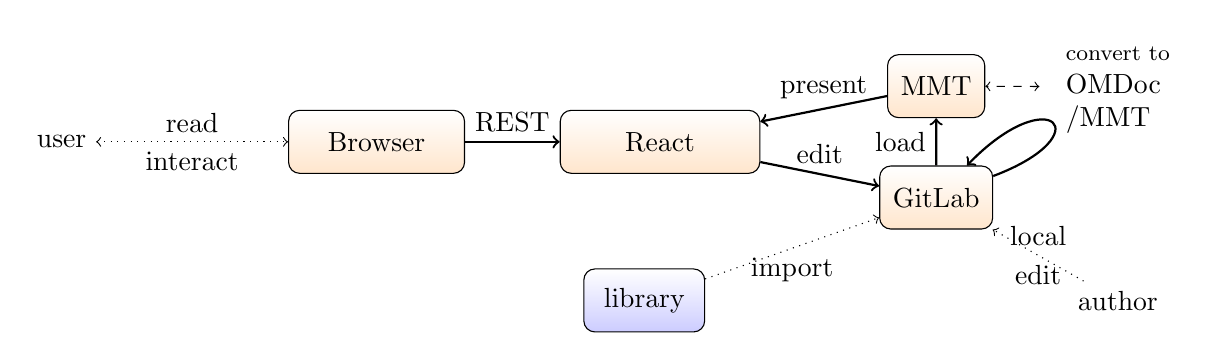
\begin{tikzpicture}[xscale=\myxscale,yscale=\myyscale]
  \tikzstyle{system} = [rectangle, draw, fill=orange!20, text width=1cm, text centered,
                                    rounded corners, minimum height=.8cm,shade, 
                                    top color=white, bottom color=orange!20]
   \tikzstyle{database} = [rectangle, draw, fill=blue!20, text width=1.3cm, text centered,
                                    rounded corners, minimum height=.8cm,shade, 
                                    top color=white, bottom color=blue!20]
\node (user) {user}; 
\node[system,right of =user,text width=2cm, xshift=3cm] (browser) {Browser}; 
\node[system,right of= browser,text width=2.3cm, xshift=2.6cm] (drupal) {React};
\node[system,above right of =drupal, xshift = 2.8cm] (mmt) {MMT};
\node[system,below right of =drupal, xshift = 2.8cm, text width=1.2cm] (gl) {GitLab};
\node[database,below left of =gl, yshift = -0.6cm, xshift = -3cm] (lib) {library};
\node[below right of =gl, yshift = -0.6cm, xshift = 1.6cm] (author) {author}; 
\node[below right of =mmt, yshift =0.7cm,  xshift = 1.6cm] (conv) {\begin{tabular}{l}\footnotesize convert to\\ OMDoc\\/MMT\end{tabular}};
\draw[<-,thick] (mmt) -- node[left]{load} (gl);
\draw[<->,dotted] (user) -- node[above]{read} node[below]{interact} (browser);
\draw[->,thick] (browser) -- node[above]{REST} (drupal);
\draw[->,thick] (gl) to[loop left,out=20,in=45,looseness=11] (gl); 
\draw[<->,dashed] (conv) -- (mmt);
\draw[<-,thick] (drupal) -- node[above]{present}(mmt); 
\draw[->,thick] (drupal) -- node[above]{edit}(gl); 
\draw[->,dotted] (author) -- node[above]{local} node[below]{edit} (gl);
\draw[->,dotted] (lib) -- node[below]{import} (gl);
\end{tikzpicture}
\caption{MathHub architecture}
\end{figure}
\ednote{look for author and user pictures}

The React based frontend that is displayed in the browser is written in TypeScript.
The use of Semantic UI React achieves an informal theme throughout MathHub.info.
The React frontend is in constant communication with an MMT server \ednote{MMT MathHub Plugin} that provides the user with the actual content as well as several semantic services.


Whereas React is used for the presentation of the content documents, GitLab is used for their versioned storage.
There the documents are organized into their proper repositories and converted from their source formats into OMDoc/MMT.
These documents can be edited in a working copy of the GIT repository.
Afterwards the author can submit the changes.

\subsection{Communication with the Backend}

As previously mentioned the frontend does not have any actual content.
It gets the data from the MMT backend.
The frontend has several clients that each communicate with a part of the server when their specific functionality is needed.
The different clients are:
\begin{itemize}
\item a Library Client for everything related to the content of the library
\item a Glossary Client that gets all the terms in a specific language
\item a Translation Client that is used by the Math Dictionary to search for a translation of a term 
\item a News Client
\item a Log Client
\end{itemize}

The answers that are received from the backend use the JavaScript Object Notation (JSON).
The data objects in JSON consist of attribute-value pairs and arrays.
The frontend then uses these objects as props for React components.


\section{MathHub Library Components}
In this section the implementation of the different components of the MathHub library is discussed.
The first page of the library is a list of all the groups of MathHub.
Every group is rendered in its own React component that has the name of the group, a short teaser and links to the corresponding group-page.

\subsection{Groups}
Above the numerous archives the group page starts with a header that has the same structure for every group.
It begins with a button that links to its source files on GitLab.
After that follows a description that gives an overview of the groups content.
The header ends with a list of e-mail addresses of the people that maintain the group. \ednote{can be seen in figure ...}

Beneath that there is a list of all the corresponding archives.
Every archive is its own React component that consists of a name and a short teaser that summarizes its content for the user.
By clicking on an entry the user is taken to the corresponding archive-page.
\begin{figure}[H]
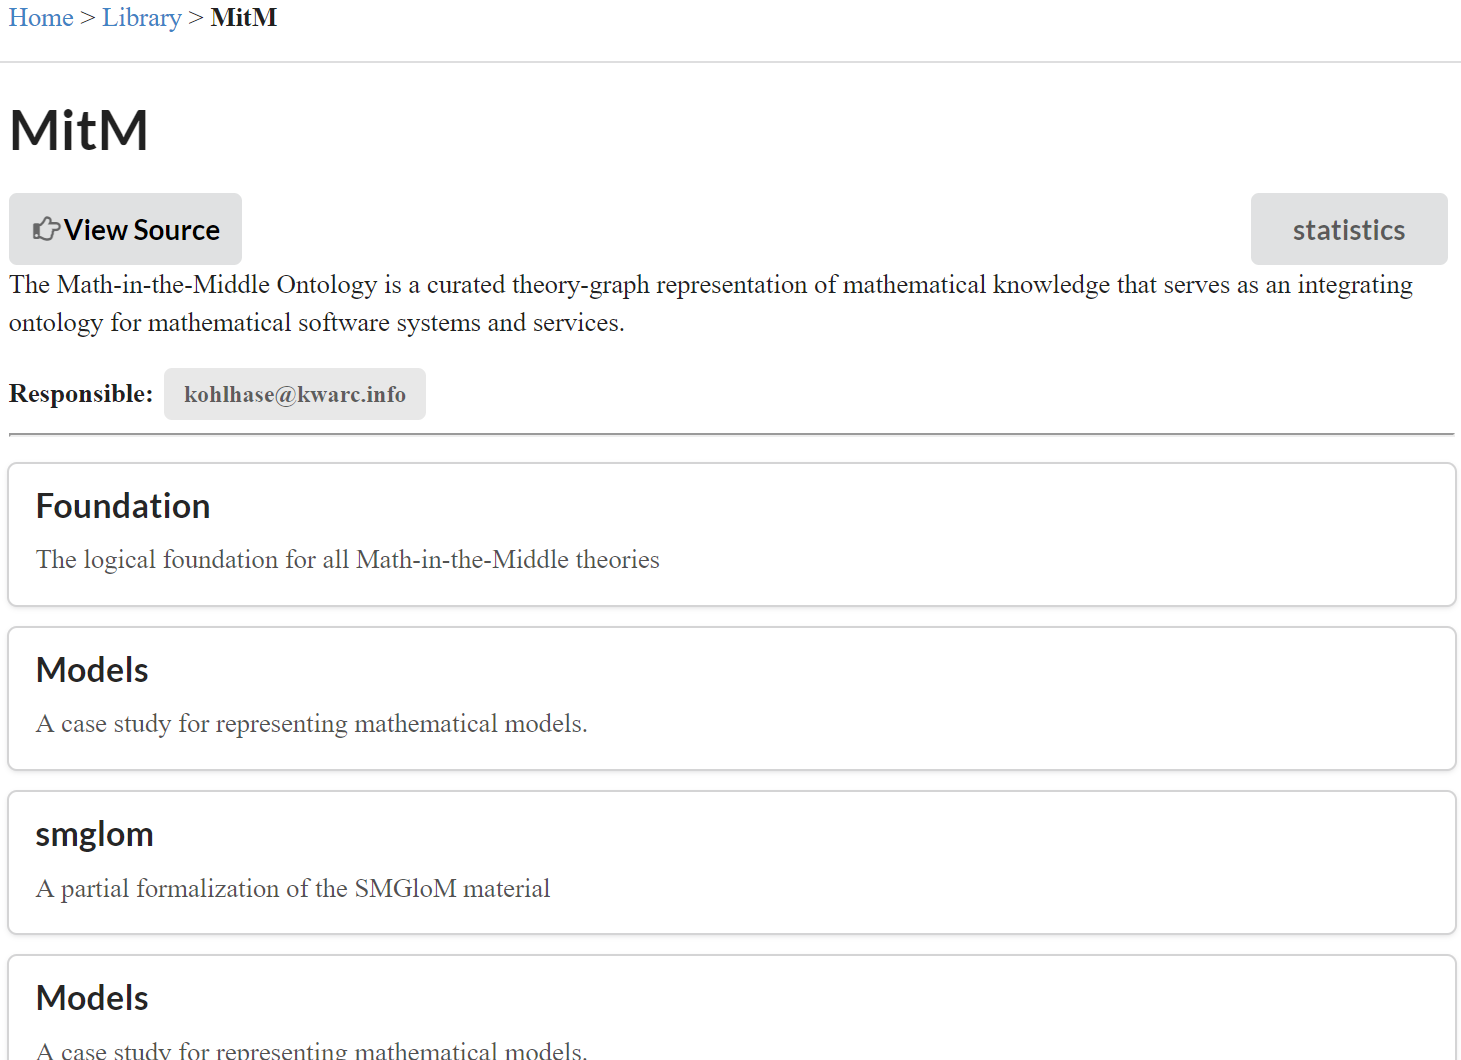
\includegraphics[width=1\textwidth]{group.png}
\caption{a group in the frontend}
\end{figure}

\subsection{Archives}
The structure of the archive-page is very similar to the group-page.
It also starts with a header that consists of a button that links to the source files, a description of the archive and the e-mail addresses of the responsible people. \ednote{can be seen in figure ...}

After the header follows a list of the documents in that archive.
There is the main difference between the group-page and the archive page.
The document entries do not have a teaser text so they just link to the document-page.
\begin{figure}[H]
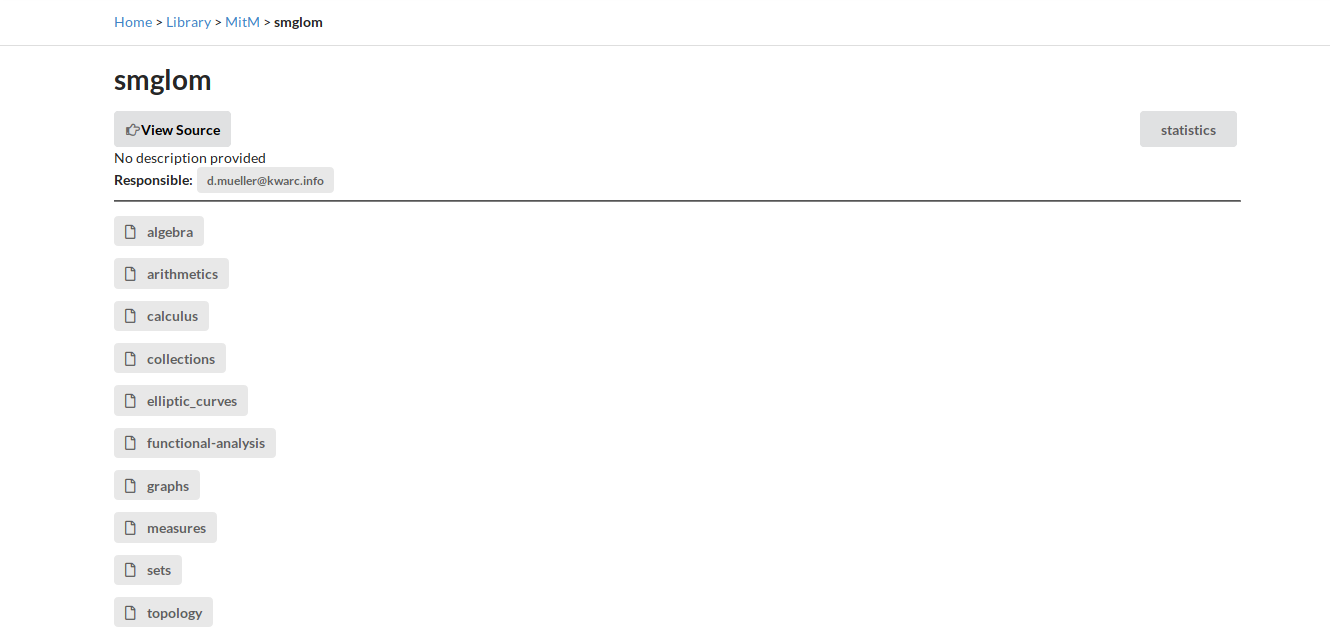
\includegraphics[width=1\textwidth]{archive.png}
\caption{ an archive in the frontend}
\end{figure}

\subsection{Documents}
Depending on the document the document-page can be either a list of OMDocs or the different modules of an OMDoc. \ednote{mix of document and module links}
If the document is in the OMDoc format there is also a button that links to its source file on GitLab. \ednote{+ jupyter}
The modules of a document are expandable React components that consist of a name, a type, either theory or view and a button to show further details.
Clicking on the button shows all the declarations and nested theories inside of a module.
These declarations (structure elements or constants) and theories can be further extended to show their own content. \ednote{can be seen in figure ...}

In between the modules there can be opaque elements.
These are just text that help the user to understand the content of the document and do not serve any contribution to the actual theories. \ednote{they are the informal part of MMT}
\begin{figure}[H]
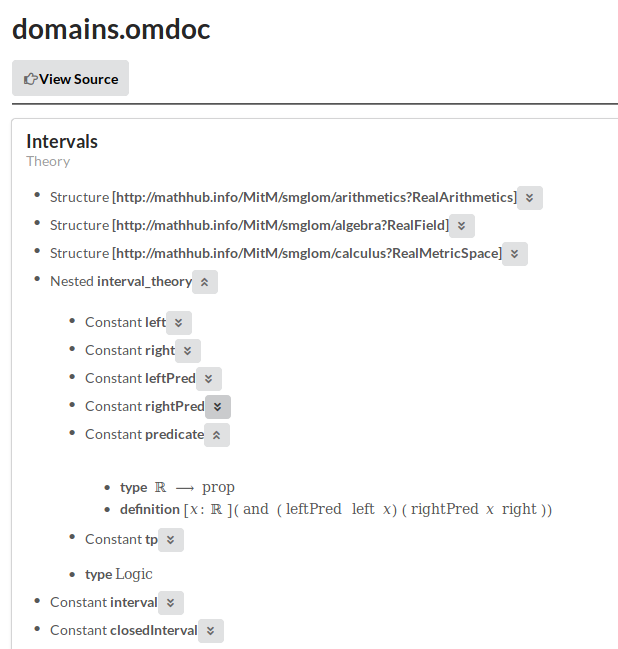
\includegraphics[width=1\textwidth]{document.png}
\caption{a document in the frontend}
\end{figure}

\subsection{Statistics}
On every group-, archive- and document-page there also is a statistics button that shows some available statistics about that particular group, archive or document.
When the cursor hovers over a keyword of a statistic that keyword is explained in a pop-up. \ednote{can be seen in figure ...}
\begin{figure}[H]
\centerline{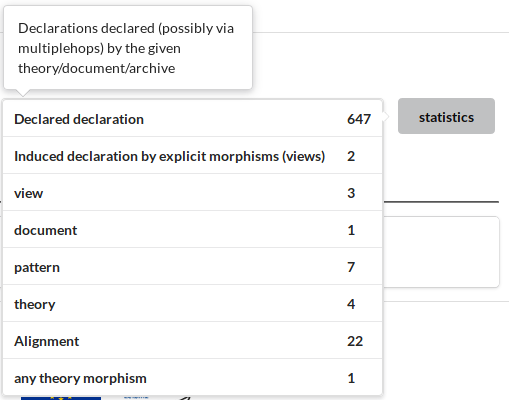
\includegraphics[width=0.6\textwidth]{statistics.png}}
\caption{statistics in the frontend}
\end{figure}

\section{The Applications of MathHub}

\subsection{Glossary}
The glossary-page has a tab for every available glossary.
At any given time only the terms are rendered that have an entry in the currently selected language.
Thus it is possible to change languages by either changing the language tab or clicking on a language-button inside an entry.
If there is a button with a different language available, this means this particular entry also exists in that language.
To create a better overview the definition of a term is not immediately shown.
By clicking on an entry the definition becomes visible. \ednote{can be seen in figure ...}
\begin{figure}[H]
\includegraphics[width=1\textwidth]{glossary.png}
\caption{the glossary in the frontend}
\end{figure}

\subsection{Math Dictionary}
To translate a term with the help of the Math Dictionary the user has to select the language from a dropdown menu in which the term currently is and also the language to which it should be translated into
Pressing the "translate" - button sends a translation request to the server.
Until the servers responds, the message "translating" is shown and the button is disabled to prevent sending to many translation requests.
If a translation exists then the translated term, its definition and potential synonyms are shown.
By selecting the same language for "from" and "to" the Math Dictionary can also be used to get the definition for an expression without searching the glossary. \ednote{can be seen in figure ...}
\begin{figure}[H]
\includegraphics[width=1\textwidth]{dictionary.png}
\caption{the Math Dictionary in the frontend}
\end{figure}

\section{Conclusion}
 \ednote{re-iterate everything}
\section{Future Work}
Obviously the work on a project like MathHub.info is never completely finished.
There are still many features left that would be a great addition to the frontend to improve the practicality and the overall user experience. \ednote{sounds to trivial?}
The biggest expansions that will be added to MathHub.info in the near future are TGView and MathWebSearch.

	\subsection{TGView} 
	TGView is a graph viewer with the task to visualize the relations between multiple theories to give a better overview over a system like MathHub.
	 The distinctive feature of TGView is that it is entirely browser based. \ednote{backend to frontend}
	 That means that its graphical interface is build on the client side to avoid sending a server request every time the user interacts with the interface, eg move or hide nodes.
	 Otherwise it would be required to refresh the page on every single change to the graph. 	\cite{tgview}
	 
	 To successfully integrate TGView into MathHub.info it is necessary to build a new React component from the existing JavaScript code.
	 
	\begin{itemize}
	\item did the old MathHub.info have tgview? => seperate MMT webpage, only now integrated
	\item browser based Graph viewer
	\item client side building to avoid page refresh when user changes the graph (eg hides nodes)
	\item has a graphical interface for actions with mouse without server requests
	\item javascript
	\item visualize theory relations for better understanding
	\item need to be build as a react component to be integrated into MathHub.info
	\end{itemize}
	\subsection{MathWebSearch}
	Explanation needed!
	\subsection{Subset Frontends}
	\subsection{Issue report: MathHub and content}
	\subsection{Jupyter Integration}

\printbibliography
\ednote{use this: github.com/KWARC/bibs/kwarc.bib}
\end{document}